\section[VAN]{VAN}
	\begin{equation}
	\label{eq:van}
	\begin{split}
 		w = \sum_{k=0}^n \frac{C_k}{(1+r)^k}
	\end{split}
	\end{equation}
	ci possiamo, quindi, calcolare il valore del \ac{TIR} corrispondente. Per definizione il \ac{TIR} è pari a:
	\begin{equation}
	\label{eq:tir}
	\begin{split}
 		\sum_{k=0}^n \frac{C_k}{(1+i)^k} = 0
	\end{split}
	\end{equation}	 

	L'andamento del \ac{VAN} in funzione dei flussi mensili è rappresentabile dalla seguente formula, calcolata tenendo conto del \textbf{tasso di sconto} $r$ pari a (\ref{eq:wacc_tax_value}):	
	\begin{eqnarray}
	\label{eq:andamento_van_flussi}
 		y(x) & = & 10,7528 \cdot ( x - 60\thinspace 131,27 ) - 56\thinspace 170,20		\nonumber \\
 			 & = & 10,7528 \cdot x - 702\thinspace 749,72
	\end{eqnarray}

 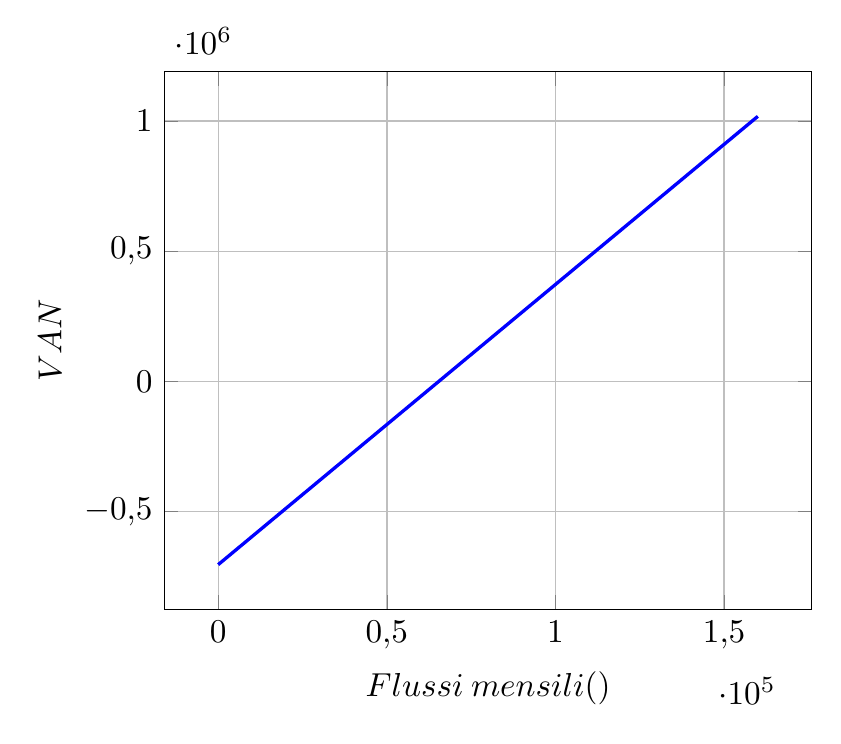
\begin{tikzpicture}[scale=1.2]
 \pgfkeys {
			/pgf/number format/.cd,
			set decimal separator={,{\!}},
			set thousands separator={}}
	\begin{axis}[ xlabel=$Flussi\: mensili (\mbox{\euro})$, 
				   ylabel=$VAN$, 
				   grid=major ]
		
		\addplot[domain=0:160000, color=blue, line width=1pt]{10.7528 * x - 702749.72};
		
	\end{axis}
\end{tikzpicture}

Un punto importante della funzione \ref{eq:andamento_van_flussi} è quello per cui il $ VAN = 0 $, ovvero:

	\begin{equation}
	\label{eq:van_zero}
	\begin{split}
 		y(x) = 0
 	\end{split}
	\end{equation}

Il valore $x$ corrispondente è pari alla quantità di flussi di cassa mensili minimi che dovremmo avere per rendere il progetto remunerativo. Il valore del flusso di cassa per cui è soddisfatta \ref{eq:van_zero} è, ponendo:
			
	\begin{equation}
	\label{eq:van_pareggio_1}
	\begin{split}
 		10,7528 \cdot x - 702\thinspace 749,72 = 0	
 	\end{split}
	\end{equation}			

pari a:
			
	\begin{eqnarray}
	\label{eq:van_pareggio_2}
		x & = & \frac{702\thinspace 749,72	}{10,7528}	 	\nonumber \\[1.5ex] 
		  & = &  65\thinspace 355,04 \: \mbox{\euro} 
	\end{eqnarray}


\usepgfplotslibrary{fillbetween}

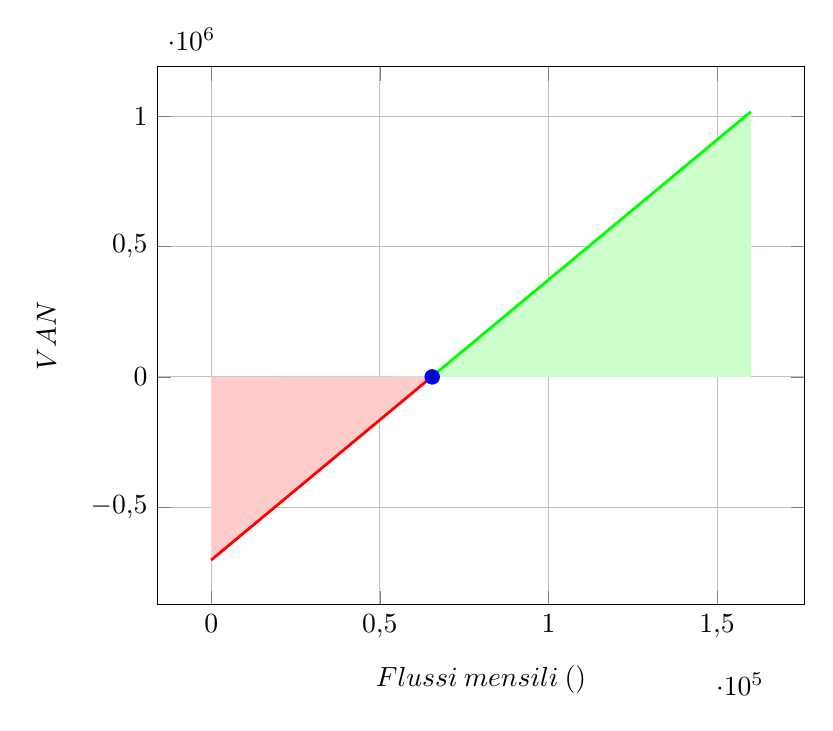
\begin{tikzpicture}[scale=1.2]
 \pgfkeys {
			/pgf/number format/.cd,
			set decimal separator={,{\!}},
			set thousands separator={}}

    \begin{axis}[thick,smooth, xlabel=$Flussi \: mensili \:(\mbox{\euro})$, ylabel=$VAN$, grid=major]    

		\addplot coordinates{( 65535, 0) };
							  
        \addplot+[domain=0:65535, name path=A,red,line width=1pt, no markers] {10.7528 * x - 702749.72};
        \addplot+[domain=65535:160000, name path=C,green,line width=1pt, no markers] {10.7528 * x - 702749.72};
        \addplot+[domain=0:160000, name path=B, draw=none,black, no markers] {0};

        \addplot[domain=0:65535, red!20] fill between[of=A and B];
        \addplot[domain=65535:160000, green!20] fill between[of=C and B];
    \end{axis}
\end{tikzpicture}


\begin{comment}
\subsection[Break-even period]{Break-even period}
	Si analizza, infine, il \textbf{punto di pareggio}, ovvero la quantità di chiamate necessarie per avere un fatturato tale da ricoprire l'investimento iniziale, in modo tale da chiudere il periodo di riferimento senza perdite né profitti.

Il \textbf{break even period} (periodo di pareggio), ovvero il periodo di tempo necessario per il recupero dell'esborso iniziale è quindi pari a:   	
\end{comment}
%
%	Tabella relativa al caso teorico in cui non ci siano malati durante un anno
%
\begin{savenotes}
\begin{table}[htb]
\centering
 \caption{Variazione VAN (Caso Teorico)}
 \begin{tabular}{p{4cm}D{,}{,}{5.2}D{,}{,}{5.2}D{,}{,}{5.2}D{,}{,}{7.4}}
 \toprule
 	& \multicolumn{1}{c}{Flusso di cassa mensile (\euro)} & \multicolumn{1}{c}{Contratti Mensili } &\multicolumn{1}{c}{\textbf{VAN}}&\multicolumn{1}{c}{\textbf{ \% Contratti}} \\
 \midrule	
	\makebox[4cm][r]{Ottimo} & 553\thinspace 419,36 & 8\thinspace 138,52 & 5\thinspace 248\thinspace 057,65 & 1,0000\\
 	\makebox[4cm][r]{Pareggio} & 65\thinspace 355,07 & 939,18 & 0,00 & 0,1154\\ 
 \bottomrule
 \end{tabular} 
\end{table}
\end{savenotes}